\documentclass[10pt,a4paper]{article}
\usepackage{amsmath}
\usepackage{amsfonts}
\usepackage{amssymb}
\usepackage{graphicx}
\usepackage{amstext}
\usepackage{url}
\usepackage[table]{xcolor}
\usepackage[font=scriptsize, center]{caption}



\title{Datagram Congestion Control}
\author{R. van Tonder, 15676633 \\ A. Esterhuizen, 15367940}
\date{\today}

\begin{document}
\maketitle
\newpage

\section{Overview}
\subsection{Description}
DCCP is an emerging protocol that aims to provide improved congestion control
alongside the TCP protocol. While its development has gone through many
phases, it is still not yet deemed ready for industry adoption. 
\paragraph{}
In this report we will investigate the characteristics of DCCP and evaluate its
effectiveness in comparison to the TCP and UDP protocols. It must be noted that
this may not accurately reflect the final, intended operation of the DCCP
protocol. This report derives value from the fact that the protocol was tested
on Linux (Ubuntu) machines whose kernel support the DCCP protocol in
its current state.

\subsection{Goal}
\label{goals}
The goal of this report is to investigate the operation of the DCCP protocol and the congestion control that is afforded
by its use. For this reason, we evaluated DCCP's operational behavior when run concurrently with both the TCP and UDP protocols. 
The three major areas of investigation are as follows:
\begin{itemize}
\item Contention of bandwidth between the TCP and DCCP protocols
\item Whether UDP suppresses the complete bandwidth of TCP and DCCP
\item Whether TCP or DCCP contends more effectively against UDP
\end{itemize}
In answering the above, the outcome of this investigation is to evaluate the effectiveness of DCCP as currently available through 
selected Ubuntu distributions. 


\section{Implementation}
The three protocols were implemented in Python. A server and client python program was written for each
of respective protocols. Simulating transmission of data over the protocols therefore involved running a
separate process for each server on a node. Furthermore, single or multiple clients corresponding to these
servers may be run on the same or different nodes.

\subsection{Features Included}
The clients can successfully connect to their respective servers, and send messages. These messages consisted of packets
of pre-determined size so as to maximize bandwidth usage of the protocol or client. In the case of DCCP, multiple clients were required
to make use of a greater amount of bandwidth, due to a variety of complications. See \S\ref{complications} for more. 

\subsection{Features Not Included}
The client implementations of the protocols do not allow multiple clients to be launched through one
execution of the program. Thus, a user may have to run the program multiple times in terminal, or otherwise
seek to make use of a bash script for doing so. This feature was not strictly required for the investigation, however.

\subsection{Extra Features Included}
The server programs provide a real-time graph of data received through its protocol. This feature was found \emph{not} to impact the
data collection significantly. For instance, saving the data instead of plotting it in real time-yielded similar bandwidth read-outs
from the servers, indicating that the act of plotting did not affected the bandwidth throughput. 
\paragraph{}
The form of data collection measured the actual data sizes of the packets received by the servers. Consider that another metric 
would be to count the number of packets received by the server, and consequently multiply it by the pre-determined packet sizes
in order to determine bandwidth usage. This latter metric was found to be a bit wanting, as it does not exhibit cases where a number
of packets may be received by the adaptor, but for various reason would not be passed up the protocol stack to the Python program. See
\S\ref{complications} for more. 

\subsection{Algorithms and Data Structures}
To ensure thread-safe operations, the use of the Python GIL (Global Interpreter Lock) was employed. This granted us
the ability to use thread-safe data structures containing the number of bytes received in a certain time period. 

Real-time graphing was enabled by appending the most current bandwidth sampling in a time interval (typically 1 second)
to a list of the 100 most recently sampled data points. The oldest data point in this list was consequently popped off.

Critically, these operations takes place in a designated thread. A \texttt{BandwidthMonitor} class was created for the purpose
of sampling the bandwidth usage in a time interval. The interval is determined by the time taken between calling the class's 
\texttt{initiate} and \texttt{terminate} methods. A lock of the bandwidth count is obtained once during each call, and the
bandwidth determined is returned by the \texttt{terminate} method.

\section{Protocol Details}
An outline of each of the protocols are given below, and the features provided by each. 

\paragraph{TCP}
TCP is a \emph{connection-oriented} protocol that ensures reliable delivery of data over a network through bit streams. Key features
that TCP provides are ordered data transfer, retransmission of lost packets, error-checking, flow control, and congestion control. 
These features allow TCP to be considered ``reliable''. 

Most of the features mentioned make use of the fact that TCP implements a sliding
window for sending and receiving data. Congestion control is afforded by four algorithms, namely, slow-start, congestion avoidance,
fast retransmit, and fast recovery. 

\paragraph{UDP}
UDP is a \emph{connectionless-oriented} protocol that does not rely on handshaking like TCP. It is considered ``unreliable'' as it 
does not guarantee delivery of UDP datagrams (or messages) that are sent to a host. Furthermore, UDP does not implement
any error-checking algorithms.

UDP is preferable to TCP in cases where waiting for packets is less desirable than dropping a few packets. UDP inherently provides
shorter latencies, and thus has application in VoIP and online games. 

\paragraph{DCCP}
DCCP is a \emph{message-oriented} protocol, and provides a reliable connection between hosts. 
The distinguishing feature of DCCP is that it it implements congestion control mechanisms at the transport layer,
 rather than assuming such control at the application layer.

This form of congestion control is considered TCP-friendly, meaning that it contends fairly in terms of bandwidth with programs making
use of the TCP protocol. However, in an application like VoIP, it is desirable to send new data rather than resend old data. Timing
constraints are placed on data in the DCCP protocol, allowing it to discard data that is considered ``too old'' to be considered
useful. 

DCCP makes use of congestion control algorithms which have a corresponding identifier. These CCID modules are implemented by
the kernel of the operating system. 


\section{Methodology and Experiments}
The investigation was carried out by considering DCCP's interaction with TCP and
UDP in turn, while keeping the goals mentioned of
\S\ref{goals} in mind.
%clients and servers terminated to determine...?

\subsection{TCP and DCCP Contention}
\label{tcpdccp}

Consider the following graphs, which give a clear indication of bandwidth fluctuation when running TCP and DCCP 
concurrently:

\newpage

\begin{figure}[!h]
\begin{center}
\hspace*{-65pt}
\includegraphics[scale=.52]{screens/re/Screenshot-33.png}
\end{center}
\end{figure}

First, a DCCP connection was made (corresponding to the blue line in the graph).
This connection consisted of three hosts running multiple
DCCP clients each, with each DCCP client sending to a single host running the
DCCP server.

After an initial 100 data points were sampled, a TCP client was launched from another
host, along with a corresponding TCP server running on the same host as the DCCP server. The new TCP connection did not
affect the DCCP connection in any noticeable way. This is likely due to the fact that the DCCP connections were
not making use of the full bandwidth available. However, note that the TCP connection is running at a lower throughput
than the approximate 117 MB/s of which it can utilize in the absence of DCCP.
\paragraph{}
Next, a series of DCCP clients were terminated. The effect of this action on TCP was a sudden rise in throughput for TCP:

\begin{figure}[!h]
\begin{center}
\hspace*{-65pt}
\includegraphics[scale=.52]{screens/re/Screenshot-12.png}
\end{center}
\end{figure}

The DCCP clients were subsequently restarted, which again resulted in a reduced throughput of TCP, as indicated above.

Following this, the behaviour of TCP and DCCP is analyzed when the initial DCCP
bandwidth
is \emph{higher} than that of TCP. Two DCCP client batches were required to
achieve this simulation. The throughput of the protocols are displayed below:



\begin{figure}[!h]
\begin{center}
\hspace*{-65pt}
\includegraphics[scale=.52]{screens/re/Screenshot-1.png}
\end{center}
\end{figure}

The above results indicate that TCP does not suppress DCCP's bandwidth when it
is in effect. Instead, TCP operates
at a lower potential throughput in DCCP's presence. After terminating one of
the DCCP client batches, TCP's throughput increased. Restarting the same DCCP
batch yielded the following graphs:

\begin{figure}[!h]
\begin{center}
\hspace*{-65pt}
\includegraphics[scale=.52]{screens/re/Screenshot-2.png}
\end{center}
\end{figure}

It is evident that DCCP's congestion control is in effect, as it allows TCP to
make use of a significant amount of bandwidth, and does not suppress it
outright. This contrasts greatly with UDP's effect as will be seen in
\S\ref{contention}.


Note also that the sum of the bandwidths used by TCCP and DCCP make use of the full spectrum of bandwidth available,
but in a controlled manner. The bandwidth spikes are considered ``anomalies'',
and are discussed in greater detail in \S\ref{complications}.


\subsection{DCCP, TCP, and UDP Bandwidth Usage}
\label{contention}
\subsubsection{DCCP and UDP}
Consider the test set-up of DCCP as above, contending for bandwidth against the UDP
protocol:

\begin{figure}[!h]
\begin{center}
\hspace*{-65pt}
\includegraphics[scale=.52]{screens/re/Screenshot-44.png}
\end{center}
\end{figure}

As indicated above, a UDP client was launched from a separate host, with the
UDP server running on the same host as the DCCP server. DCCP bandwidth
is immediately suppressed down to a minute amount of about
0.5 MB/s. 
\paragraph{}
The following scenario depicts the behavior of UDP initially running in the absence of DCCP traffic.
Note the stability of UDP bandwidth (i.e. no fluctuations), 
prior to enabling DCCP traffic.

\begin{figure}[!h]
\begin{center}
\hspace*{-65pt}
\includegraphics[scale=.50]{screens/re/Screenshot-46.png}
\end{center}
\end{figure}

After initiating DCCP traffic, UDP traffic fluctuates greatly. However, it restricts DCCP
traffic to a very small amount.

Extending this idea, consider the following graphs, which indicate the
fluctuation
of DCCP and UDP bandwidth upon successive addition of DCCP clients. In
particular, it is notable
that DCCP does not gain any additional bandwidth by enabling more clients.
\begin{figure}[!h]
\begin{center}
\hspace*{-65pt}
\includegraphics[scale=.52]{screens/re/Screenshot-48.png}
\end{center}
\end{figure}

While dips in UDP traffic are evident, DCCP's bandwidth remains
the same as the above scenario, at approximately 0.5 MB/s. However,UDP
fluctuates much more in DCCP's presence as opposed to in its absence.

Interestingly, it was discovered that in the event that the UDP
traffic is terminated while DCCP transmission (however small) is active,
DCCP will \emph{not} proceed to make use of the bandwidth that has
become available:


\begin{figure}[!h]
\begin{center}
\hspace*{-65pt}
\includegraphics[scale=.52]{screens/re/Screenshot-50.png}
\end{center}
\end{figure}

It will be seen that this contrasts with TCP's behavior when
UDP transmission is active. Thus, while DCCP has some effect
on the stability of UDP, it cannot compete fairly for bandwidth.

\subsubsection{TCP and UDP}
The scenario above is repeated with TCP replacing DCCP.
In the same vein, consider the bandwidth utilization of the TCP
and UDP protocols in the graph below:

\begin{figure}[!h]
\begin{center}
\hspace*{-65pt}
\includegraphics[scale=.52]{screens/re/Screenshot-4.png}
\end{center}
\end{figure}

As indicated, TCP bandwidth takes a sharp dive as soon as
the UDP client starts sending data. 
\paragraph{}
In the following graphs, two notable points are raised. First,
UDP bandwidth fluctuates greatly while the TCP protocol is active.
Second, UDP bandwidth stabilizes as soon as the TCP bandwidth
is eliminated:

\begin{figure}[!h]
\begin{center}
\hspace*{-65pt}
\includegraphics[scale=.52]{screens/re/Screenshot-7.png}
\end{center}
\end{figure}

However, unlike DCCP, TCP is able to make use of the available
bandwidth when UDP is terminated:

\begin{figure}[!h]
\begin{center}
\hspace*{-65pt}
\includegraphics[scale=.52]{screens/re/Screenshot-15.png}
\end{center}
\end{figure}


\section{Extra Tests and Considerations} %i want a three way battle, all-in-one
This report would not be complete without an evaluation of all three protocols
running concurrently. However, it was necessary to establish each pairing
separately, so that  the behaviour from all
three protocols can be analyzed with these results in perspective. Consider the
following three graphs which summarize the following sequence of events:

\begin{enumerate}
 \item One DCCP client batch is started, followed by a second batch
 \item A TCP client is started
 \item One DCCP client batch is terminated
 \item A UDP client is started
 \item The UDP client is terminated
\end{enumerate}

\hspace*{-65pt}
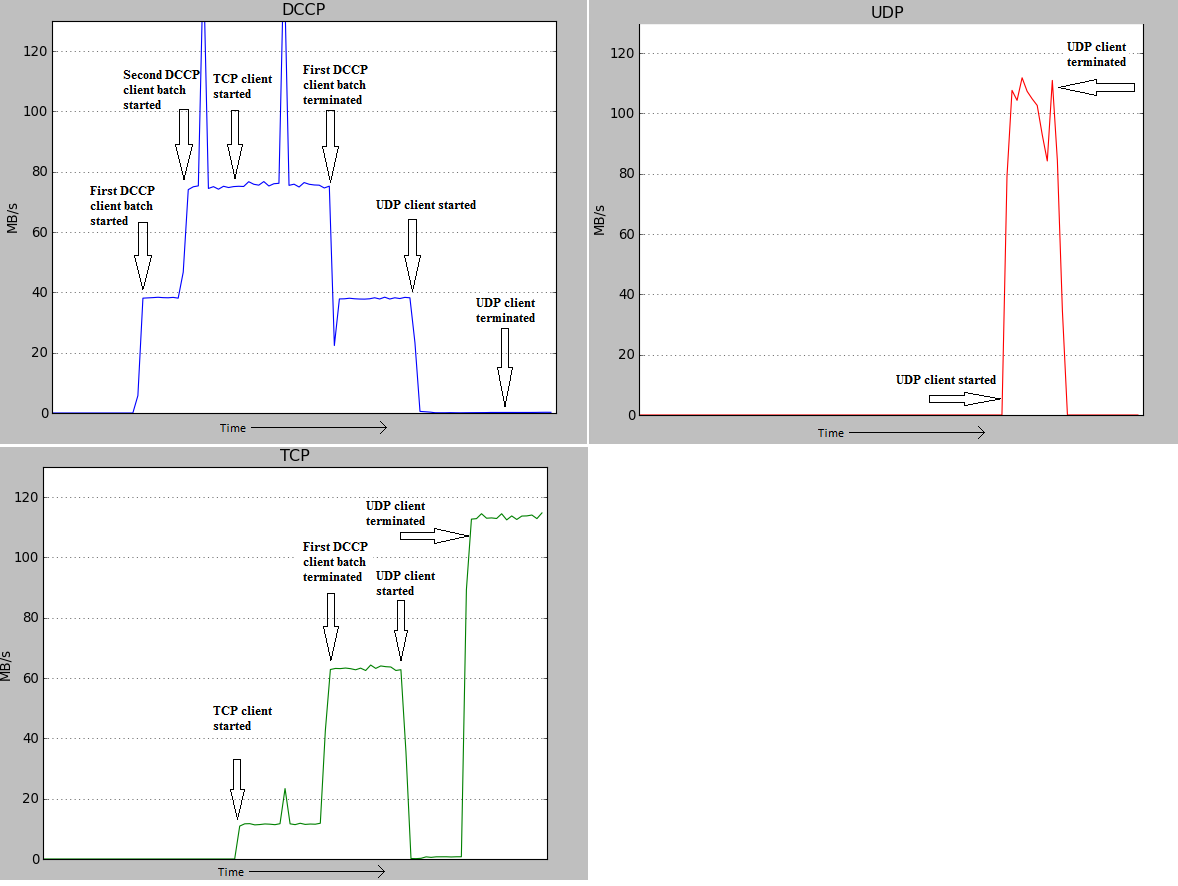
\includegraphics[scale=.52]{screens/trio.png}

The following behaviour is notable, and confirms the results found in the
previous sections.

\begin{itemize}
 \item When DCCP consumes the majority of the bandwidth initially, the
initialized TCP client can still operate at with a reasonable amount of
bandwidth available.
 \item When one of the DCCP client batches is terminated, TCP's bandwidth
raises actively.
 \item The immediate presence of UDP traffic suppresses both that of TCP and
DCCP's bandwidth.
 \item After the UDP client is terminated, TCP is able to make use of the
available bandwidth, while DCCP is not. 
\end{itemize}


\section{Results}

Having considered all of the above cases, the results can now be delivered
conclusively.
\paragraph{}
Firstly, in \S\ref{tcpdccp} it was confirmed that DCCP tolerates TCP traffic to
a
much better extent than UDP. If TCP initially has a greater amount of incoming
traffic, DCCP throttles itself accordingly. If DCCP initially has a greater
amount of incoming traffic, TCP is still able to operate at a reasonable level.
\paragraph{}
Secondly, in \S\ref{contention}, it was established that UDP indeed suppresses
TCP and DCCP traffic. However, it does not completely and utterly do so, as
TCP and DCCP can operate at a very ineffective level of about 0.5 MB/s. 
\paragraph{}
Finally, it was interesting to note that while neither TCP or DCCP can hinder a
large amount of incoming UDP traffic, only TCP can ``recover'' \emph{after} the
UDP traffic stops. DCCP traffic, on the other hand, remains at the very low
rate that UDP suppressed it to.
\paragraph{}
The reason behind this latter point is not absolutely clear. One speculated
reason is that the congestion control behind DCCP throttles DCCP traffic only
in relation to TCP traffic, and not UDP. Thus, where DCCP can effectively
maintain a reasonable bandwidth while only TCP is running, it has no safeguards
once there is UDP traffic incoming. Once this UDP traffic is eliminated, DCCP
does not detect that it has stopped, and maintains a low throughput.

\section{Problems and Interesting Findings}
\label{complications}

\subsection{Establishing a DCCP connection}
One of the problems we\footnote{The authors are fully aware
that the use of personal pronouns are employed in this section. This is because
``we'' performed and encountered these actions. This is assumed to be an
appropriate tone, and should not be considered ``colloquial''.} experienced was
DCCP's inability to establish a connection
without user intervention. 
\paragraph{}
In order to establish a DCCP connection from a client to
a server on different computers, it was first necessary to attempt a connection both ways. 
That is, one would need to initialize clients on both computers, each attempting
to connect
to the other. This connection need not succeed, but 
is necessary in order to prompt the kernel to use DCCP.
These clients, their role being fulfilled, are
discarded. Only then can a client-server connection from one computer to the
other succeed.

\subsection{Error 11}
There were some initial difficulties in sending data over a DCCP connection. We initially
simply sent our data using \texttt{socket.send()} on the client side, believing
that as with TCP
and UDP, this would be sufficient. This would result in \texttt{socket error
11, resource currently
unavailable} being thrown, implying that if congestion is high, the congestion
control 
protocol can decide not to send the data.
\paragraph{}
The \texttt{send} statement was thus placed within a try-except
block a long with a sleep statement. The sleep statement would pace the client
and prevent
congestion, while the try-except block would ensure that the client
continued to  to send data after the ``resource unavailable'' exception
occurred. 
\paragraph{}
All that remained was to fine-tune the amount of time that the client would
sleep for. Smaller times resulted
in higher throughput and larger times resulted in lower throughput. It was hoped that there would be
an ideal duration of time that would prevent the congestion control protocol from blocking the client,
but ultimately the sleep interval was kept small to keep throughput high.

\section{Conclusion}



\end{document}
